\documentclass[11pt]{article}
\usepackage{hyperref, graphicx, float, caption} 
\captionsetup{justification=raggedright, singlelinecheck=false}
\graphicspath{{./pics/}}
% Title Page
\title{Assignment 1 - MPP: Message-Passing Programming}
\author{Marian Daogaru, 25685252}
\date{09/05/2017}
\usepackage{geometry}

\geometry{a4paper,
	total={170mm,257mm},
	left=20mm,
	top=20mm,}

\usepackage{fancyhdr}
\pagestyle{fancy}
\fancyhf{}
\rhead{Marian Daogaru, 25685252}
\lhead{FEEG6003}
\cfoot{\thepage}

\usepackage{listings}
\usepackage{color}
\definecolor{dkgreen}{rgb}{0,0.6,0}
\definecolor{gray}{rgb}{0.5,0.5,0.5}
\definecolor{mauve}{rgb}{0.58,0,0.82}
\lstset{frame=tb,
	language=C,
	aboveskip=3mm,
	belowskip=3mm,
	showstringspaces=false,
	columns=flexible,
	basicstyle={\small\ttfamily},
	numbers=none,
	numberstyle=\tiny\color{gray},
	keywordstyle=\ttfamily\color{blue},
	commentstyle=\color{dkgreen},
	stringstyle=\color{mauve},
	breaklines=true,
	breakatwhitespace=true,
	tabsize=3
}

\begin{document}
	
	\maketitle
	\pagebreak
	\tableofcontents
	\pagebreak
	
	\section{Serial Program}
	
	In this report, Message Passing using MPI shall be presented. The main aim is to create a program able to reconstruct an image from an initial compressed image, such as Figure \ref{pic0}. The program should divide the image into smaller parts, assign each chunk to different processes, create the new image, and finally reconstruct the image. 
	
	Firstly, we should look at the serial case. The serial program, with only one process running, should create a good first basis for reconstructing the initial image. In addition, it will give us a benchmark for comparison between the serial case and the 2D case. 
	
	The main code for the serial part can be seen in Appendix B (\ref{ap2}). Initially, the code is able to accept argument if passed, otherwise it would use the default values. The arguments refer to the size of the picture, the number of iterations at which $\Delta$ and the average pixel value are calculated, and the maximum value of $\Delta$ under which the process should stop. 
	We refer to $\Delta$ as the difference between two consecutive values of a pixel. Thus, it is the change in value after an iteration.
	
	\begin{figure}[H]	
		\centering
		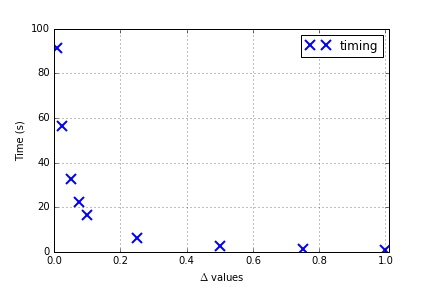
\includegraphics[scale=0.5]{serialvs3.jpeg}
		\caption{Execution time for the serial code for different values of $\Delta$.}\label{serial3}
	\end{figure}
	
	Now, after arguments were passed, the code would read the initial values of the pixels into an array of size MxN. In addition, a new array of size M+2 x N+2 would be created, such that the new edges (halos) would be assigned the value 255 (maximum for 8bit) for reconstruction. The next step is to calculate the value of each pixel into a new array from an \textit{old} array, calculate $\Delta$ and the average, assign the new values to the \textit{old} array, and repeat until finished. For this program, the exit conditions of this would be either to achieve a maximum number of iterations (100,000 was set as maximum), or if the maximum $\Delta$ calculated would be smaller than a limit value. Lastly, after the loop was finished, the new image would be reconstructed. A new value of a pixel would be created using the given equation:
	$$new_{i,j} = \frac{1}{4}(old_{i+1,j} + old_{i-1,j} + old_{i,j+1} + old_{i,j-1} - edge_{i,j})$$
	
	The maximum value of iteration was chosen as 100,000 as it can be seen in Figures \ref{avg1} and \ref{avg2} that, although those picture are for the 2D case the values for the average are identical for serial and 2D, the average value of a pixel follows a logarithmic curve. Thus, more iterations would not actually provide more benefit tot the overall efficiency of our simulation.
	
	Although the serial is not the main aim of this project, several timing measurements were done. Figure \ref{serial3} presents the overall execution time for the serial code for different values of $\Delta$. The program either exited the main loop after the maximum number of iterations was achieved, of the maximum $\Delta$ went below the limit. It can be seen that execution time follow an exponential curve, which is to be expected as the the program exits the loop later, and the improvement has an exponential decrease, as presented above. For our example, Figures \ref{pic5} and \ref{pic1} present the 768 x 768 pixel image for different values of $\Delta$. While in the second picture, $\Delta=0.05$, being 5 times higher than in the first picture, there is not much visual difference between them. Consequently, a stopping criteria based on $\Delta$ is critical for not wasting time and resources for a small improvement.
	
	Figure \ref{serial4} present the relative time of execution for the serial, when $\Delta$ is calculated at a certain number of iterations, compared to when it is not calculated. When not calculated, the loop will finished at the highest iteration, thus the longest execution time. It can be observed, as expected, that the more $\Delta$ is calculated, more time is required for execution. At higher number of iterations, there is almost no difference between the number of iterations it takes. Figure \ref{serial5} presents how calculating the average affects the execution time, similar to the previous case. It can be seen again that the more time we calculate it (at smaller intervals), more execution time is required. From these graphs, it was concluded that initially, a $\Delta=0.05$, number of iterations for calculating $\Delta$ and the average of 100, would be a good trade-off between speed-up and accuracy. However, the same measurements have to be done for the parallel case. The initial assumptions for these timing values were $\Delta=0.05$, number of iterations for calculating $\Delta$ of 100 and number of iterations for calculating the average of 200. 
	
	\begin{figure}[ht]	
		\centering
		\begin{minipage}[b]{.5\textwidth}
			\centering
			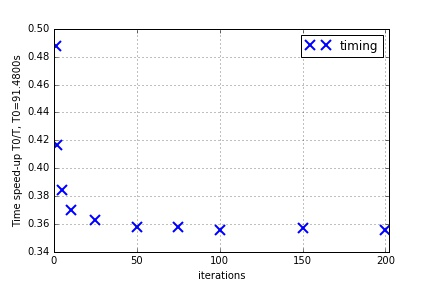
\includegraphics[width=\linewidth]{serialvs4.jpeg}
			\caption[short]{Relative execution time for different intervals at which $\Delta$ was measured. $T_0$ for no measurement.}\label{serial4}
		\end{minipage}%
		\begin{minipage}[b]{.5\textwidth}
			\centering
			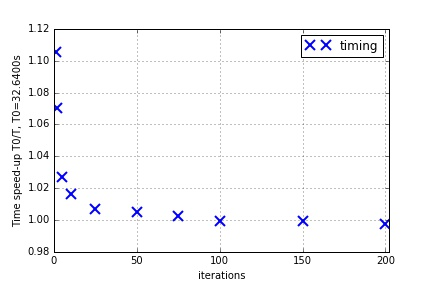
\includegraphics[width=\linewidth]{serialvs5.jpeg}
			\caption[short]{Relative execution time for different intervals at which the average was measured. $T_0$ for no measurement.}\label{serial5}
		\end{minipage}%
	\end{figure}

	\section{Two dimensional problem}
	Similar to the serial case, the source code for this Chapter can be found in Appendix C (\ref{ap3}). Additional instructions on how to compile and run the program can be found in Appendix E (\ref{ap5}).
	
	This chapter presents the architecture of the two dimensional problem for image processing. While the serial code was able to achieve the objective, the execution time was relatively slow, especially for the \textit{biggest picture}. If the an even bigger picture was given, the execution time would increase rapidly. As such, we explore another method in which the picture is split into smaller parts. Each part is then given to another process to compute, and at the end bring everything together. As such, we would be able to achieve the same results, yet in a faster time. 
	
	The general outline of this code is quite similar to the previous case: arguments are received, the buffer is read, followed by calculating pixel values over a certain number of iterations, and ending with recreating the image. Additionally, the $\Delta$  and average values are calculated at a given number of iterations.
	
	\subsection{Architecture}
	As before, we start the main execution of the program by reading the input arguments, if any are given. If not, the defaults shall be used. In this case, the arguments refer to the picture dimensions in pixel, the frequency (number of iterations) at which $\Delta$ and the average pixel value are calculated, and the maximum $\Delta$ value. As in the previous case, although we tested for that case what the optimum values should be, we shall retest for this case and confirm the optimum values for the later 3 parameters. As such, the defaults were set as 100, 200, 0.05 respectively. 
	
	Next step is represented by the initialisation of the Message Passing Interface (MPI). For the initial test, 6 processes were used. At this point, we are interested in sharing the data between processes. Firstly, the initial image data is read into an initial array, \textit{masterbuf}. Next, based on the rank (its number to distinguish between different processes), we are choosing its local buffer, named \textit{buf} in this case.  
	
	
	
	Given the fact that all the pictures are rectangles in shape, we firstly assume that each process will receive an equal number of pixels, represented by a smaller rectangle from the picture. We are interested in the case where each process works on chunks of data similar in shape with the initial data, rather than strips created by slicing the data in one dimension. As such, in order to properly compute the values of pixel at each iteration, as presented before, for every pixel we must know its neighbour. Thus besides the initial chunk of data, each buf must contain additional data (in the form of rows and columns of pixels) from its nearby processes. Consequently, to map the neighbouring processes, we start off by determining the optimum size of each buf, depending on the total number of processes. Thus process is achieved by finding the two closest integers. m and n, that multiplied would equal the number of processes running, and each integer divides with no remaining one of the dimensions of the picture. These integers define the number of rows (n) and columns (m) the image shall be split into. Having these 2 numbers, the masterbuf is divided between processes as follows: starting from left to right, the first row contains processes 0 to m-1, second row contains processes m to 2m-1, until all processes have been allocated a chunk of data. Each process receives a chunk of data of dimensions $\frac{M}{m}x\frac{N}{n} =MP x NP$. This method has its limitations, as if the sizes are not divisible by the integers, some data will be lost.
	
	After each process has received its buf, the main loop of the program starts, where the values of the pixels are calculate. Again, $\Delta$ and the average pixel value are calculated, for stopping criteria. As mentioned before, each process requires data from its respective neighbours to for a halo around its local buf in order to execute properly calculate the value of each pixel. Each process has 4 neighbours: up, down, left, or right. If its local buf has been assigned by an edge, the halo side is already assigned in preprocessing, therefore no need to swap this. However, for the remaining edges, these values must be swapped. Consequently, the actual buf of a process has a size of MP+2xNP+2.
	
	As such, each process requires to send a maximum number of 4 arrays and receive just as many. To achieve this, a communication protocol was created. For all communications, the nob-blocking asynchronous \textbf{MPI\_Isend} and \textbf{MPI\_Recv} were used. As such, to help build the halos of the left and right neighbours, a process sends the second column to the left neighbour, and the MP+1 column to the right neighbour. Moreover, it receives from the left neighbour its MP+1 column in order to replace the first local (halo region) column, and it receives from the right neighbour its first column to replace the local last column (halo region). To save time, just the elements on rows 1 to NP+1 are sent, not the halos. To achieve this communication, the actual algorithm is to use 2 \textbf{MPI\_Isend} followed by 2 \textbf{MPI\_Recv} and 2 \textbf{MPI\_Wait} at the end for actually receiving the message. If one process if faster than another, it has to wait for its neighbour to send the values for proper computation to take place.
	
	The next phase is represented by the \textit{vertical} communication: swapping the halos with the neighbours having the chunks placed above and below the local chunk. While this problem is similar to the left and right neighbour situation described above, the code was created in C. As such, for an array, elements are contiguous is memory on the Y axis, but not on X axis for a 2d array, such us the local buf or the masterbuf mentioned earlier. In the previous case, we were sending columns, thus successive elements contiguous in memory. However, for the X axis, horizontal rows are not comprised of contiguous elements in memory. Thus, in order to be able to use the \textbf{MPI\_Isend} and \textbf{MPI\_Recv}, a special sort of structure able to map the memory is needed. This is achieved by using the MPI function \textbf{MPI\_Type\_Vector} in parallel with an MPI data type. Below the command is presented. The function requires several arguments. First, the number of arrays it should send. The next argument represents the number of elements sent on each array. These elements are send from a bigger array, starting from position 0. The bigger array is the size of the third argument. Thus, looking at the example the remaining arguments are the type of data sent, and the new data type to which the map will be locked. We can see that a total of MP arrays will be created, of size 1, the first element in an NP+2 array. After the first element was chosen, NP+1 elements will be skipped before the next element is chosen. 
	
	\begin{lstlisting}
	MPI_Type_vector(MP, 1, NP+2, MPI_FLOAT, &new_array);
	\end{lstlisting}
	
	Having this structure in mind, it the same halo swap structure is done on horizontal elements (rows) between the local buf and the up and down neighbours. After the communication has ended, the normal loop is executed. When the main loop ends, either by reaching the maximum number of iterations or the maximum $\Delta$ condition, data is gathered to be written into the recreated picture. This part is achieved by having each process send their local buf to the MASTER process (rank 0). The MASTER process then will write its own part first, followed by writing the data obtained from incoming messages. The communication protocol remains the same, using \textbf{MPI\_Isend} and \textbf{MPI\_Recv}. 
	
	\subsection{Performance}
	
	Having the software created, we can now start to measure the performance. Firstly, for all tests, unless otherwise specified, the default variable are as follows: picture size 768x768, $\Delta$ = 0.05, $\Delta$ iteration frequency of 100, and average measurement iteration frequency of 200. The code was run using 6 processes. The error bar presented in the graphs is the difference in $\mu s$ between the fastest and the slowest executing process. 
	
	We start by looking at the speed-up achieved using different values of $\Delta$, with $\Delta_{benchmark}=0.01$. Figures \ref{iter3} and \ref{iter32} present the speed-up achieved. It can be seen that for close values of $\Delta$, there is a smaller speed-up compared, to high values of $\Delta$. However, the accuracy of our measurements goes down as well. It can be seen in Figures \ref{avg1}, \ref{avg2}, \ref{pic5} and \ref{pic1} that between $\Delta=0.01$ and $\Delta=0.05$, while the average continues to increase, visually all details can be observed during inspection. As such, a default value of $\Delta=0.05$ was again considered sufficient for this exercise. 
	
	\begin{figure}[H]	
		\centering
		\begin{minipage}[b]{.5\textwidth}
			\centering
			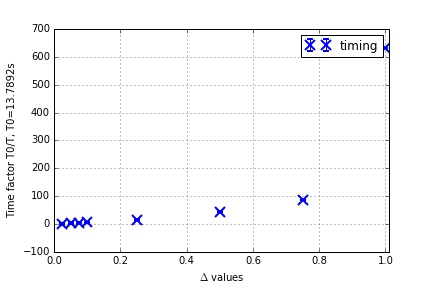
\includegraphics[width=\linewidth]{itervs3.jpeg}
			\caption{Relative execution time for different values of $\Delta$. $T_0$ is at $\Delta=0.01$.}\label{iter3}
		\end{minipage}%
		\begin{minipage}[b]{.5\textwidth}
			\centering
			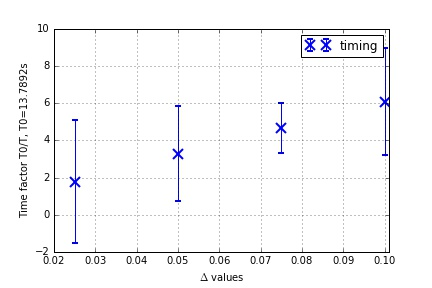
\includegraphics[width=\linewidth]{itervs32.jpeg}
			\caption{Close-up for the relative execution time vs $\Delta$ values.}\label{iter32}
		\end{minipage}
	\end{figure}
	
	Next, Figure \ref{iter4} presents the speed-up regarding the importance of calculating $\Delta$. It can observed that not calculating $\Delta$ presents a disadvantage. In addition, having an iteration frequency of 25 does not present a real advantage, it just limits the amount of data created, which can be a potentially good if storing memory is an issue. A speed up of 3.1 was observed in this case. Again, the initial assumption of an iteration frequency of 100 is considered sufficient. Lastly, Figure \ref{iter5} presents the impact of calculating the average value of pixels in the image. It can be seen that the execution time is not affected past an iteration frequency of 10. This is more than enough for our purposes. Thus, it can concluded that for consistency, the iteration frequency for calculating the average should be 100, same as the frequency for calculating $\Delta$. 
	
	\begin{figure}[ht]	
		\centering
		\begin{minipage}[b]{.5\textwidth}	
			\centering
			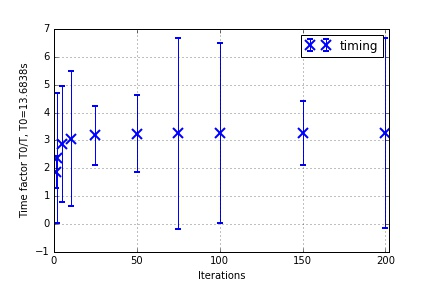
\includegraphics[width=\linewidth]{itervs4.jpeg}
			\caption{Relative execution time for different intervals at which $\Delta$ was measured. $T_0$ for no measurement.}\label{iter4}
		\end{minipage}%
		\begin{minipage}[b]{.5\textwidth}
			\centering
			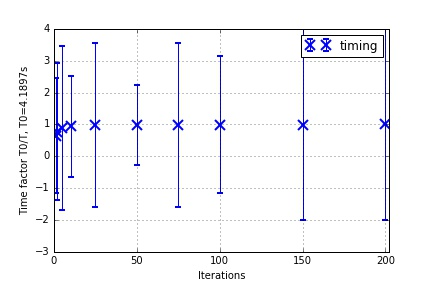
\includegraphics[width=\linewidth]{itervs5.jpeg}
			\caption{Relative execution time for different intervals at which the average was measured. $T_0$ for no measurement.}\label{iter5}
		\end{minipage}
	\end{figure}
	
	\begin{figure}[H]	
		\centering
		\begin{minipage}[b]{.5\textwidth}
			\centering
			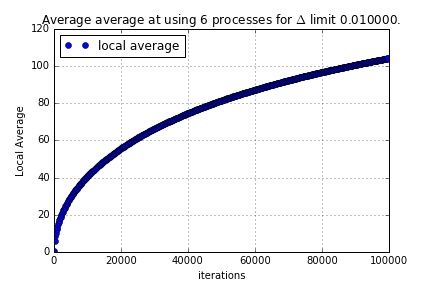
\includegraphics[width=\linewidth]{local_avg_6_010000.jpeg}
			\caption{Average value of image pixel over 100,000 iteration for $\Delta=0.01$.}\label{avg1}
		\end{minipage}%
		\begin{minipage}[b]{.5\textwidth}
			\centering
			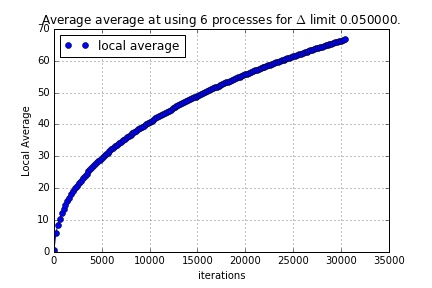
\includegraphics[width=\linewidth]{local_avg_6_050000.jpeg}
			\caption{Average value of image pixel over 100,000 iteration for $\Delta=0.05$.}\label{avg2}
		\end{minipage}
	\end{figure}
	
	
	\section{2d performance measurements}
	
	Several measurements are created to test the speed-up generated by using multiple processes. Figures \ref{exec_1}, \ref{exec_2}, \ref{exec_3}, and \ref{exec_4} present the the execution time, and the speed-up against the serial code, of the 2d algorithm for all the given pictures. The code was run for 50,000 iterations. Each picture was recreated 5 times, to check consistency. It can be seen, that for larger images, an increase in the number of processes defines an increase in speed-up. In addition, it can be observed that the increase is not linear though, but rather follows a logarithmic curve. 
	
	However, for smaller images, it can be seen that after a certain number of processes, the efficiency is decreased. Figure \ref{exec_1} presents this case quite well. Additionally, it can be seen that after this part has been reached, the consistency of the speed-up decreases, with timing by up to 10\%. The main reason for this convergence is given by the communication overheads and the size of the local buf. The more processes are communicating in a program, the more the wait time between them is increased. In addition, a smaller picture would produce smaller local bufs. With an increase in number of processes, the size of the buf would not be decreased by much. Thus, the majority of the time would be spend waiting for communication. In addition, it can be observed that for the bigger pictures have a higher speed up. This reinforces that the size of the local buf is important.
	
	\begin{figure}[H]	
		\centering
		\begin{minipage}[b]{.5\textwidth}
			\centering
			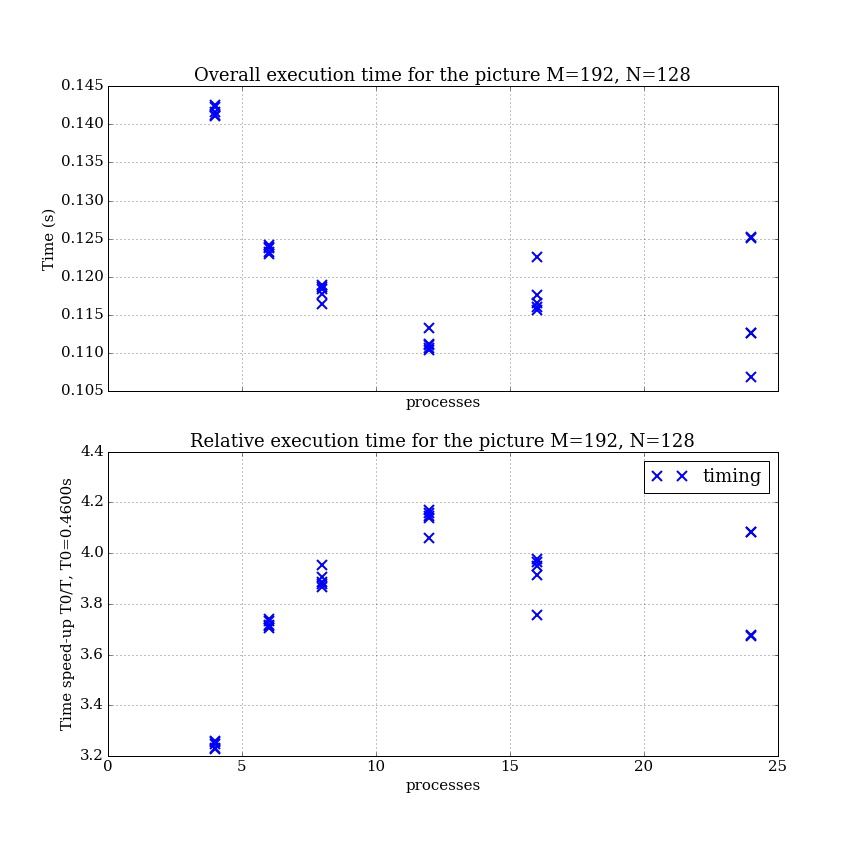
\includegraphics[width=\linewidth]{exec_192x128.jpeg}
			\caption{Execution time and relative(to serial) execution time for the 192x128 pixel image.}\label{exec_1}
		\end{minipage}%
		\begin{minipage}[b]{.5\textwidth}
			\centering
			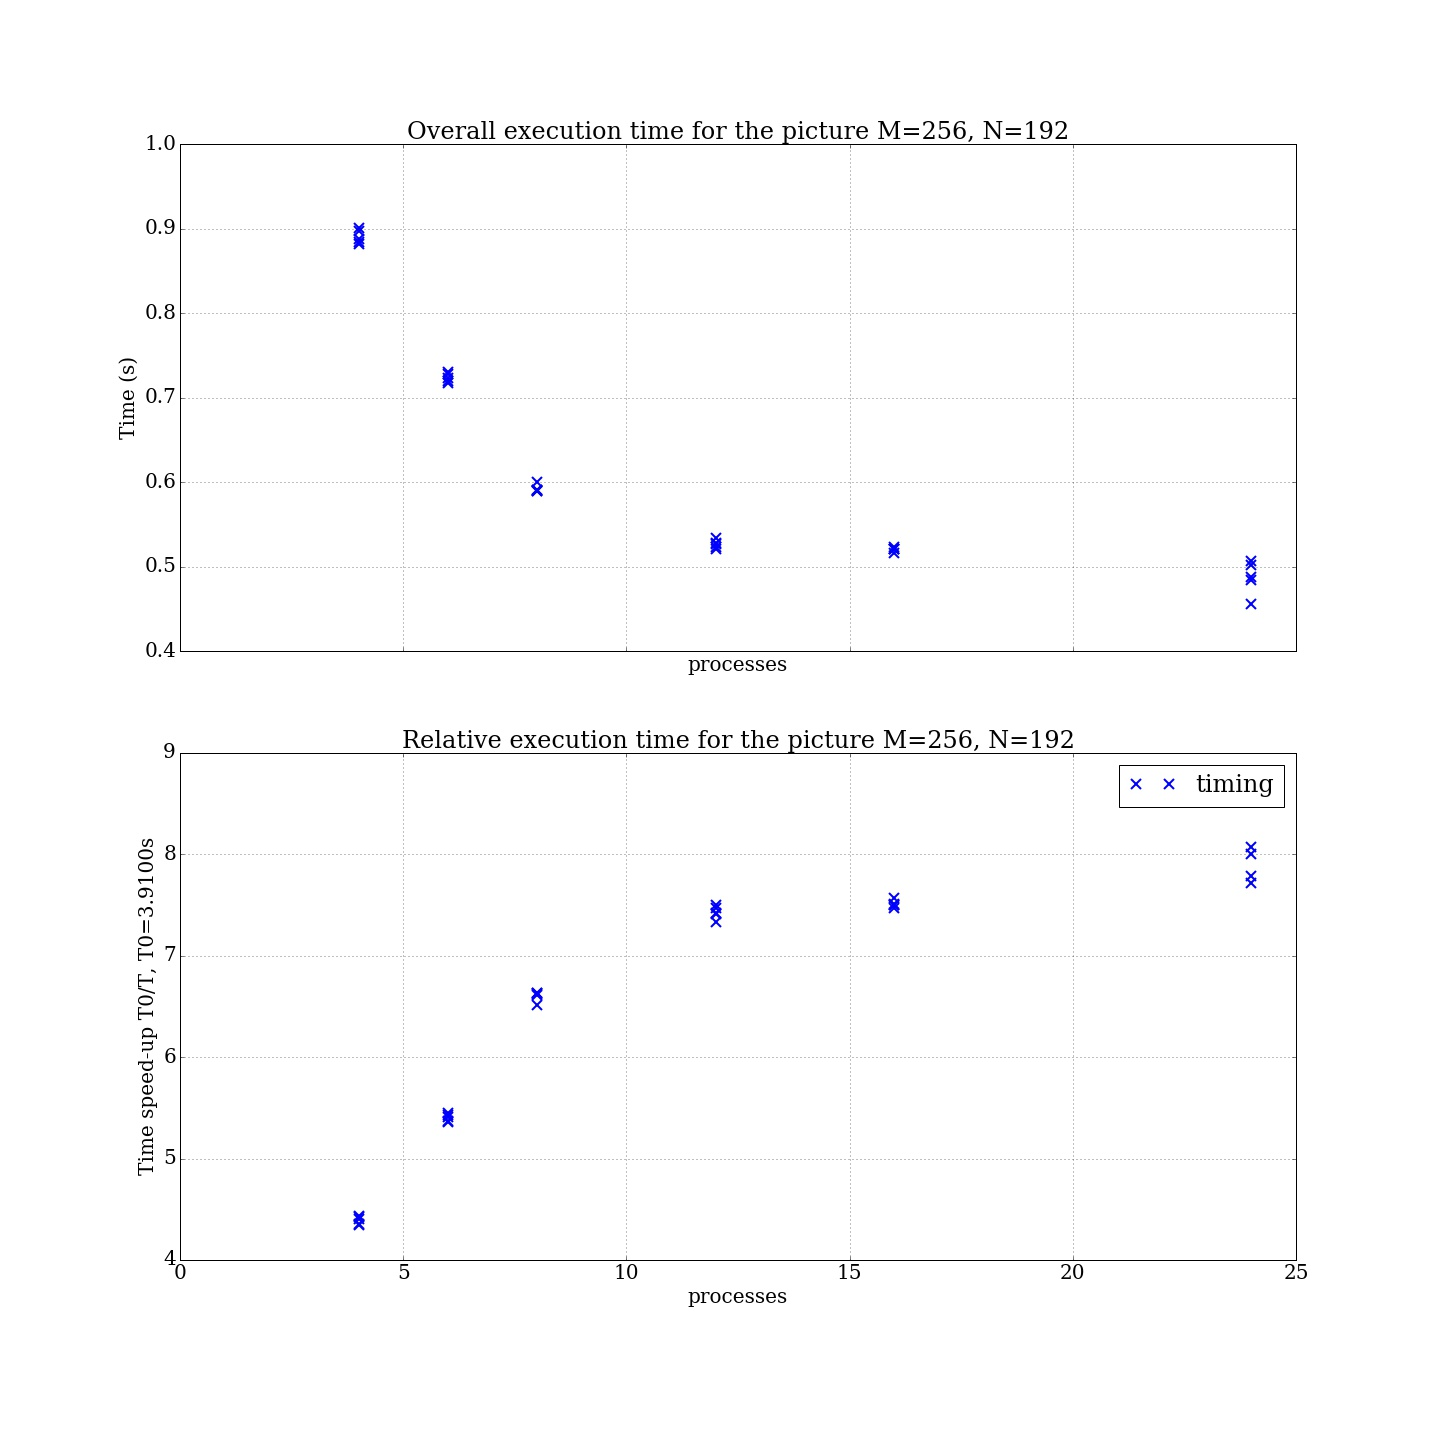
\includegraphics[width=\linewidth]{exec_256x192.jpeg}
			\caption{Execution time and relative(to serial) execution time for the 256x192 pixel image.}\label{exec_2}
		\end{minipage}
	\end{figure}
	
	\begin{figure}[ht]	
		\centering
		\begin{minipage}[b]{.5\textwidth}
			\centering
			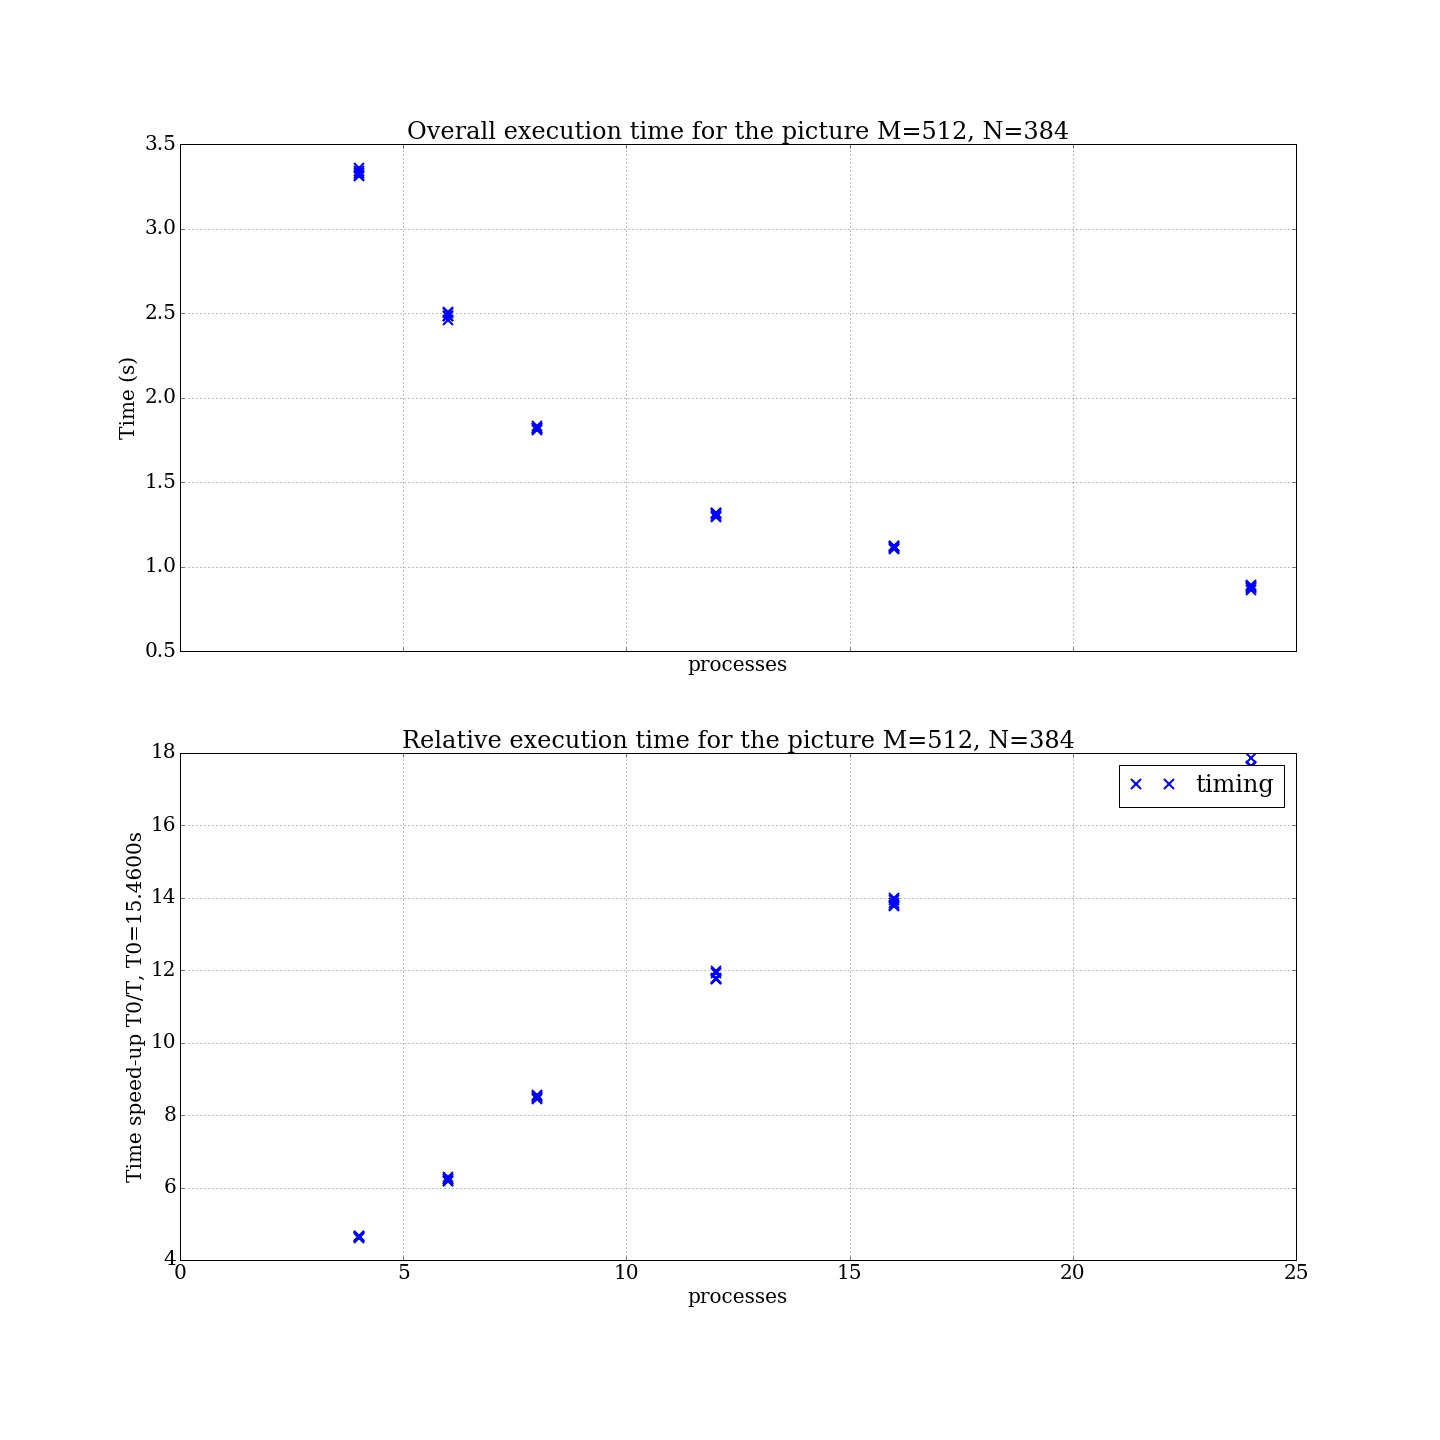
\includegraphics[width=\linewidth]{exec_512x384.jpeg}
			\caption{Execution time and relative(to serial) execution time for the 512x384 pixel image.}\label{exec_3}
		\end{minipage}%
		\begin{minipage}[b]{.5\textwidth}
			\centering
			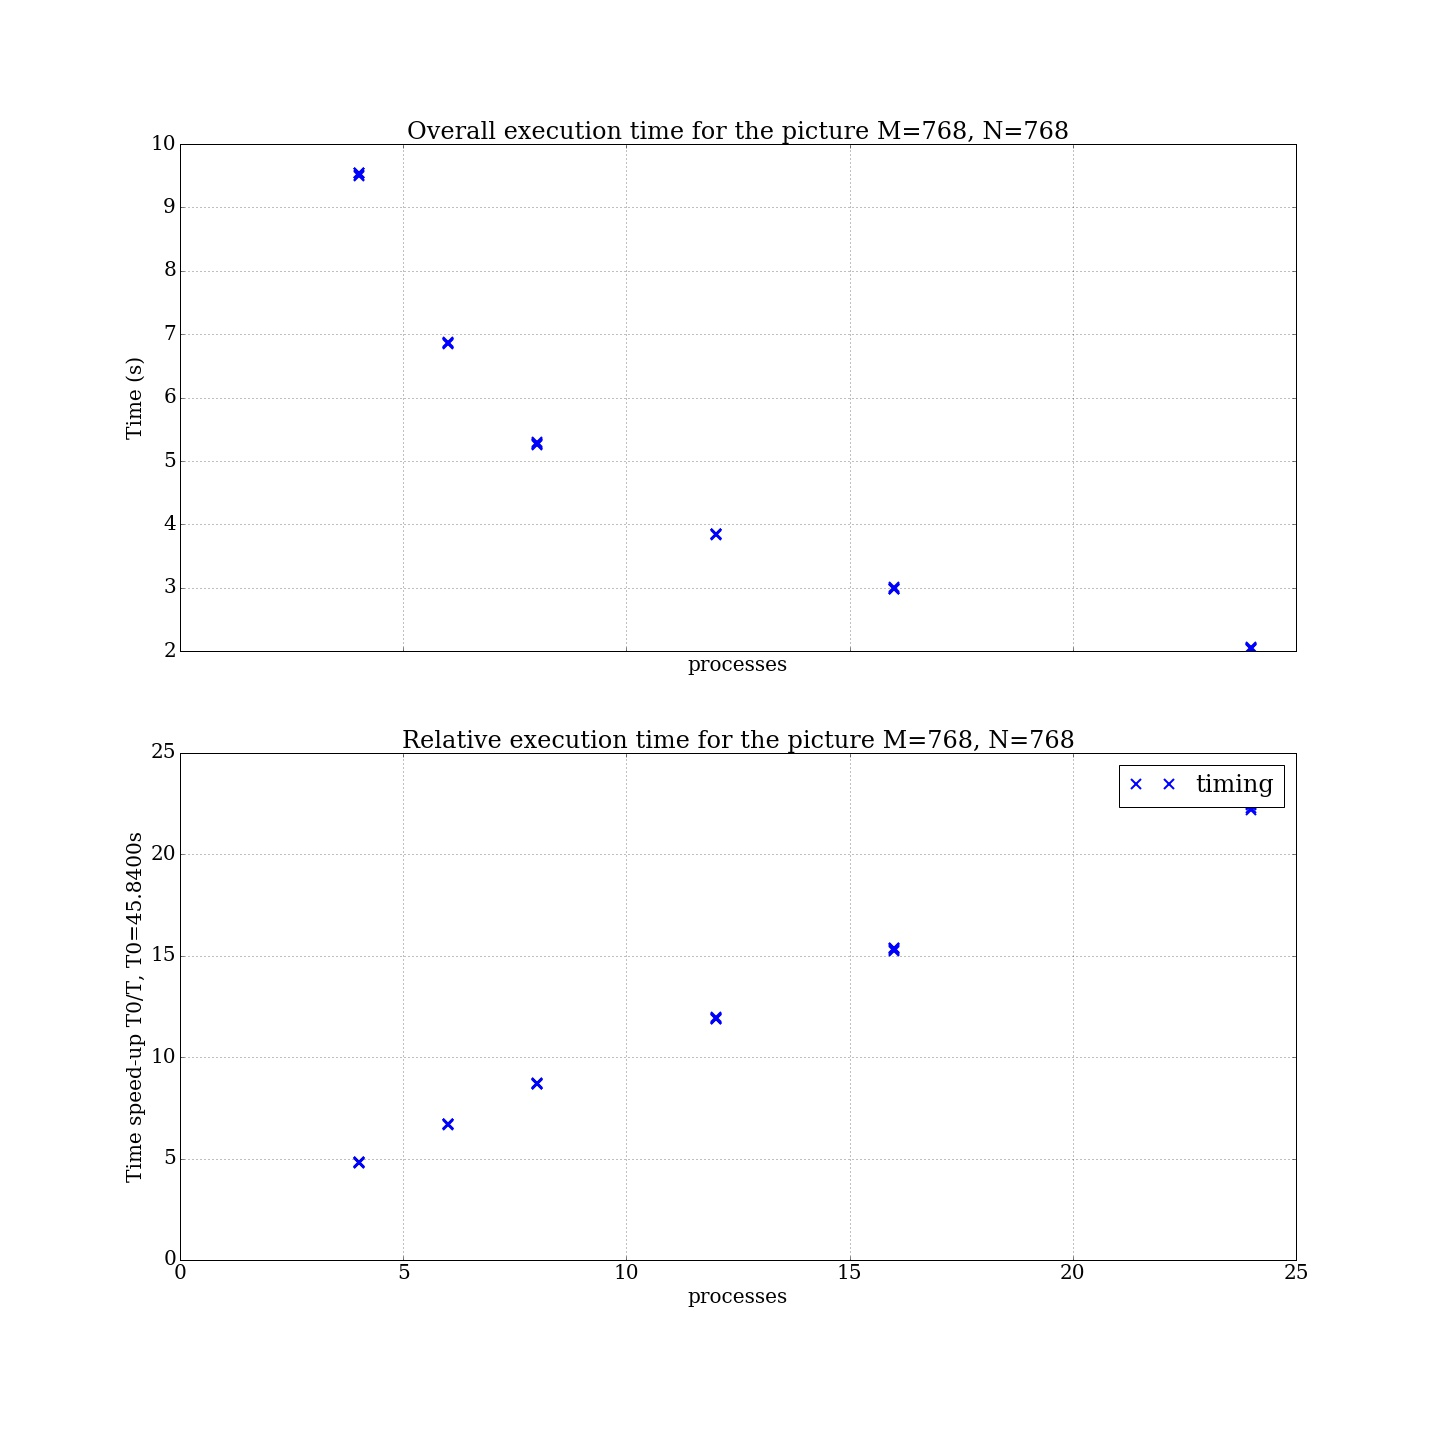
\includegraphics[width=\linewidth]{exec_768x768.jpeg}
			\caption{Execution time and relative(to serial) execution time for the 768x768 pixel image.}\label{exec_4}
		\end{minipage}
	\end{figure}

	\begin{figure}[ht]	
		\centering
		\begin{minipage}[b]{.5\textwidth}
			\centering
			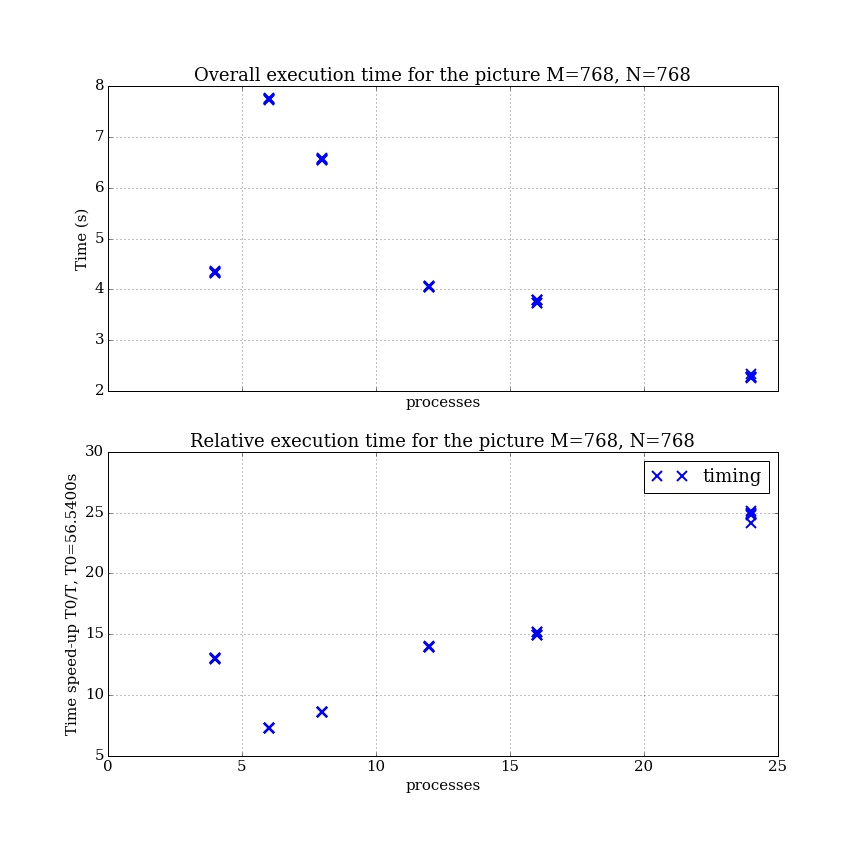
\includegraphics[width=\linewidth]{exec_768x768_odd.jpeg}
			\caption{Execution time and relative(to serial) execution time for the 768x768 pixel image.}\label{exec_4odd}
		\end{minipage}%
		\begin{minipage}[b]{.5\textwidth}
			Figure \ref{exec_4odd} presents a weird behaviour, observed just in the largest picture. Algorithm was supposed to run until a $\Delta=0.01$ was reached. It can be seen that for 4 processes, the program finished quite fast. After careful investigation, it was concluded that this was due to the actual difference between pixels being small caused by small overall progress. 
		\end{minipage}
	\end{figure}
	
	For consistency, we checked the total value of the pixels in the new image after 50,000 iterations against the initial image, for different number of threads running. It can be observed, that for the same number of iterations, the difference in consistent. Thus, the algorithm is consistent, and the more processes are running, the image is just reconstructed faster, without data loss.
	
	\begin{lstlisting}
	Threads @ delta=0.01 			4 				6 				8 				12 				16 				24 
	diff					-54968212.0	-54968212.0	-54968212.0	-54968212.0	-54968212.0	-54968212.0
	\end{lstlisting}
	
	Lastly, Figure \ref{tim1} presents several important timing measures, where the program stalled. The most important figure is represented by the average loop execution time for different number of processes. This refers to the time it took for 1 main loop to execute. It can be seen that decrease is exponential, with the increase in number of processes. As the loop will run for thousands of times, decreasing this figure represents the main method of increasing the speed up. Besides, it can be seen that mapping the neighbours (make MP) is the fastest part of the program. \textit{Make buf} represents the creation of the local buf from the master buf. This part is executed by each process only once. While it is quite fast, order of 10e-4 to 10e-7, it still decreases with the number of processes being run. The most time consuming part of the code is represented by the reconstructing of the image (\textit{reconstruct}), and waiting for all processes to have their buf reconstructed (\textit{barrier}). Again, these parts will be executed just once during the program. Thus, decreasing the execution time on purpose, given the fact their order of magnitude is similar to 10 average loops, would be counter productive. 
	
	
	\begin{figure}[H]	
		\centering
		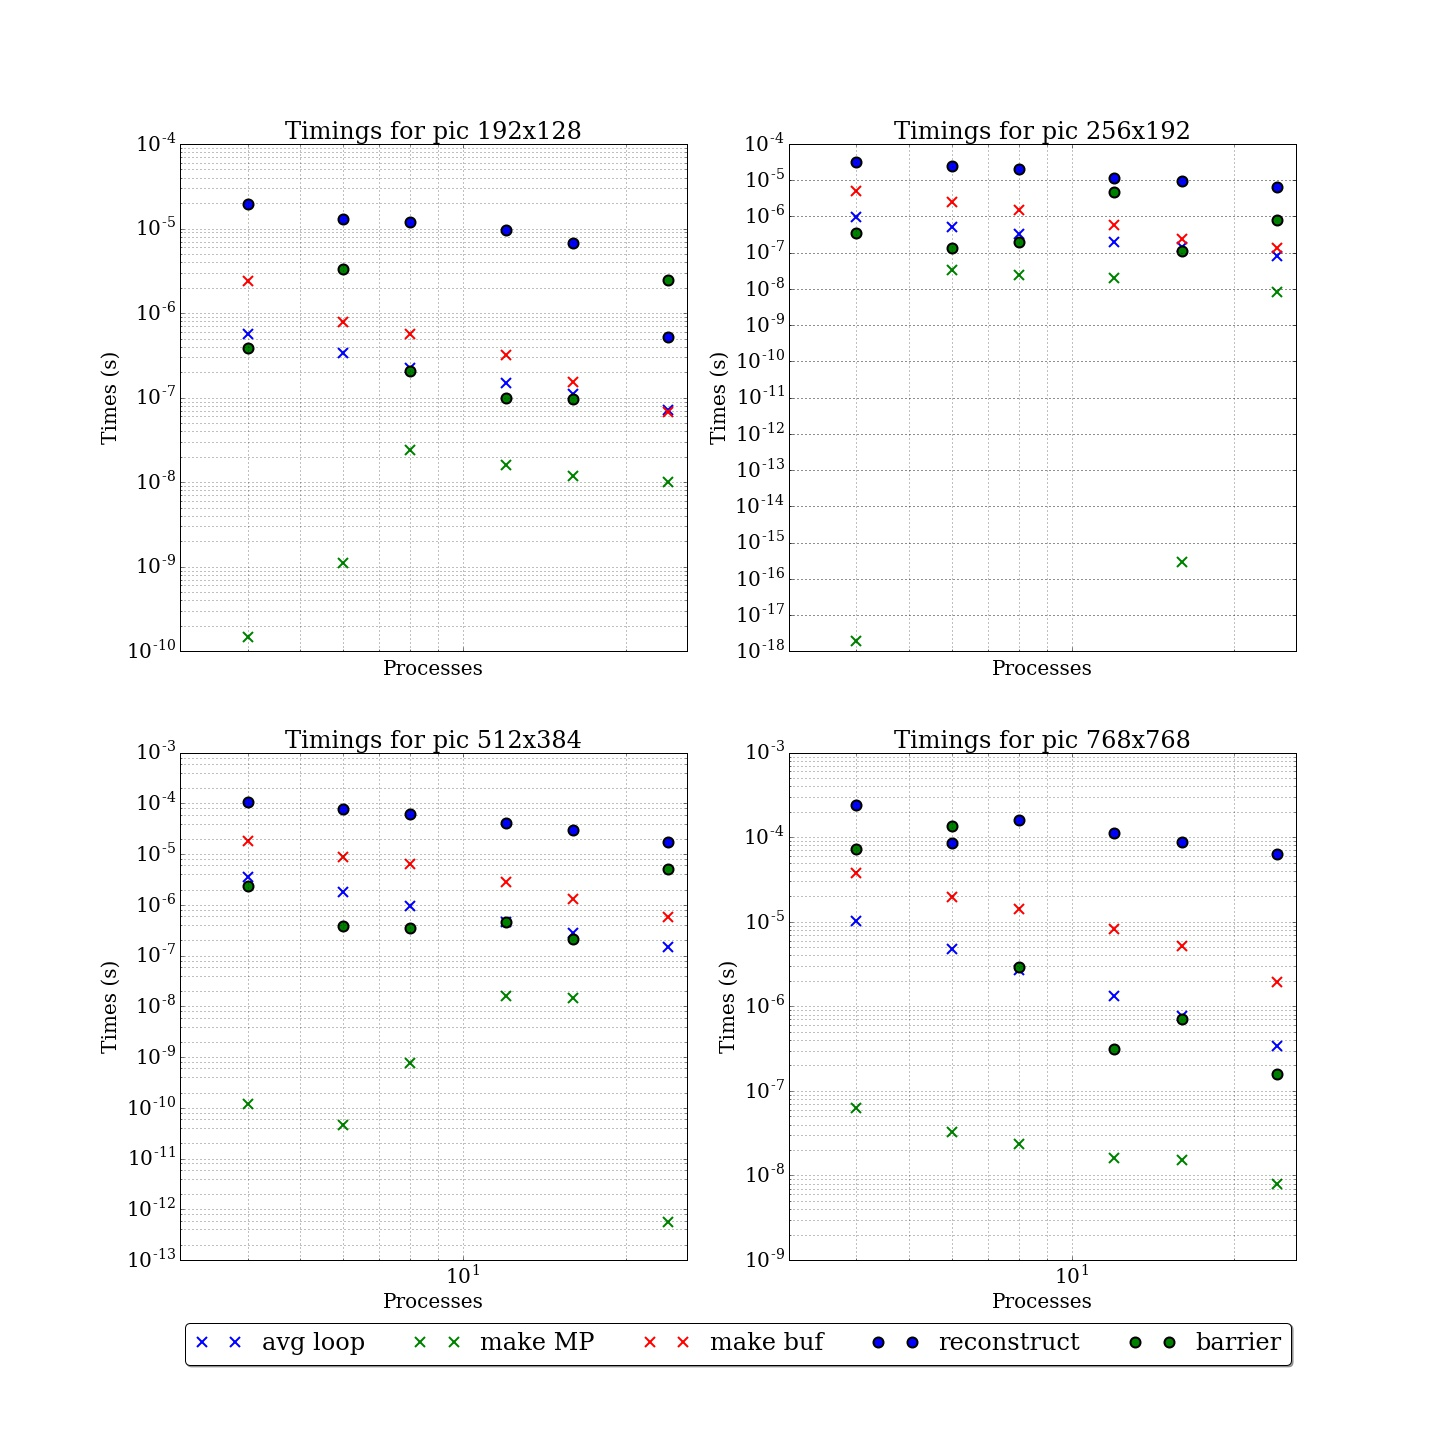
\includegraphics[scale=.3, width=\textwidth ]{timings.jpeg}
		\caption{Timing for different parts of the program with the typical parameters for different number of threads.}\label{tim1}
	\end{figure}
	
	\section{Conclusion}


	\pagebreak
	\section{Appendix A - Pictures} \label{ap1}
	
	\begin{figure}[H]	
		\centering
		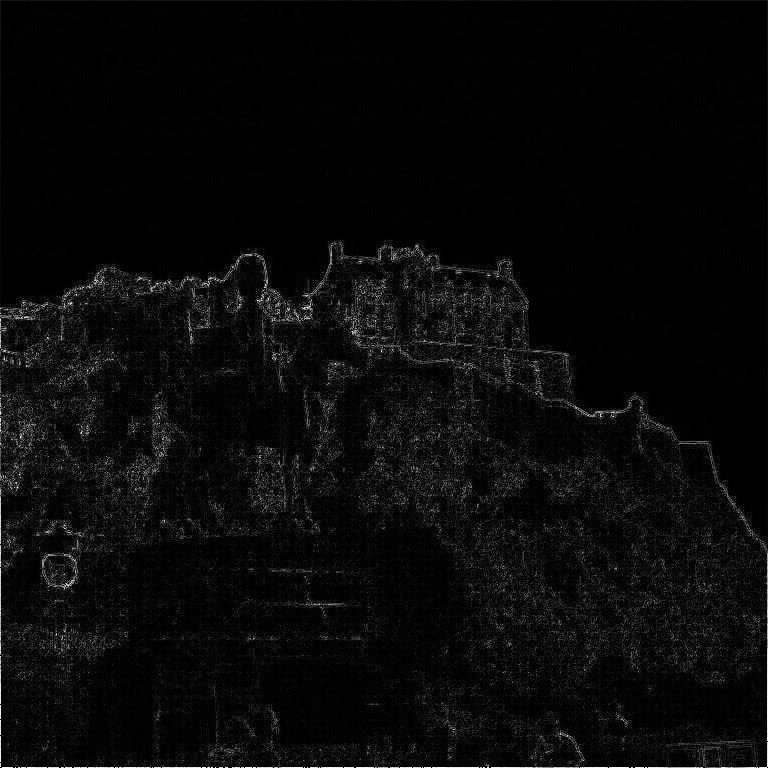
\includegraphics[scale=0.23]{edge768x768.jpg}
		\caption{Unprocessed image.}\label{pic0}
	\end{figure}
	
	\begin{figure}[H]	
		\centering
		\begin{minipage}[b]{.5\textwidth}
			\centering
			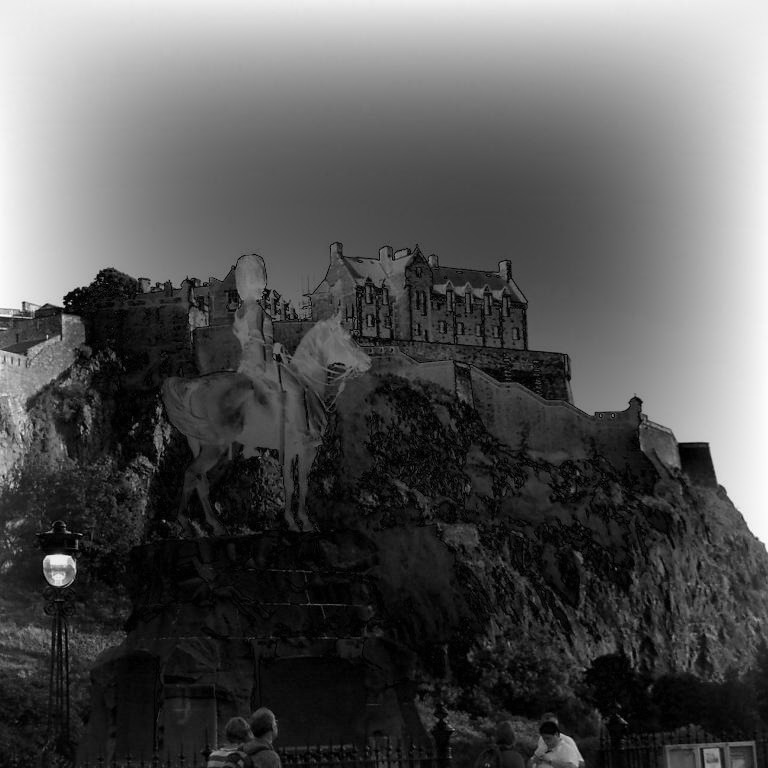
\includegraphics[scale=0.23]{edge768x768_050.jpg}
			\caption{Processed image with $\Delta=0.05$.}\label{pic5}
		\end{minipage}%
		\begin{minipage}[b]{.5\textwidth}
			\centering
			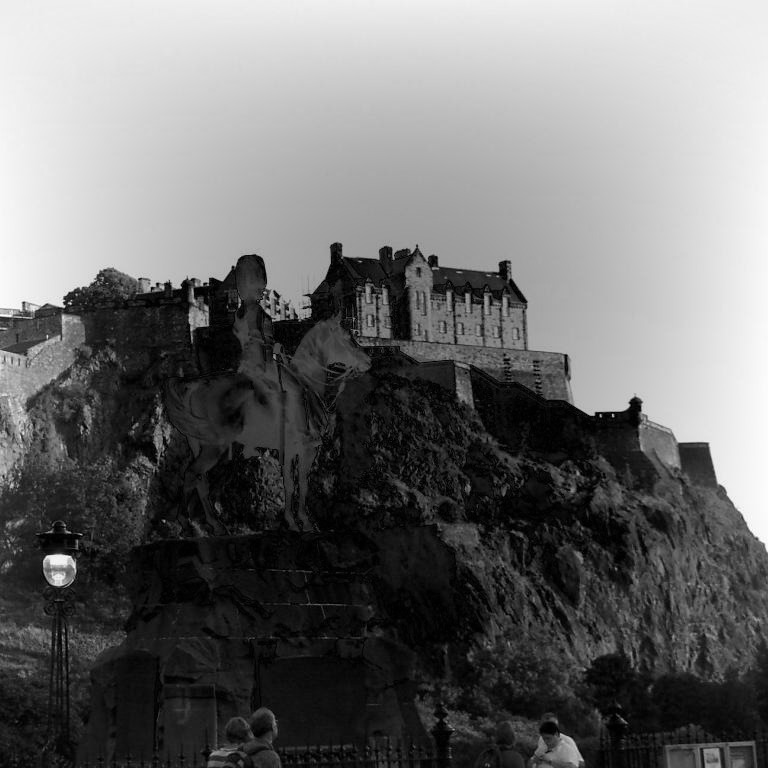
\includegraphics[scale=0.23]{edge768x768_010.jpg}
			\caption{Processed image with $\Delta=0.01$.}\label{pic1}
		\end{minipage}
	\end{figure}

	\pagebreak
	
	\section{Appendix B - Serial Code}\label{ap2}
	\begin{lstlisting}
	#include <stdio.h>
	#include <stdlib.h>
	#include <math.h>
	#include <string.h>
	#include <time.h>
	
	#include "pgmio.h"
	
	double average(double *times, int r, int iter);
	double mySum(void *myArray, int size);
	double myAverage(void *myArray, int size);
	float maxValue(float *myArray, int size);
	double avg_time(double *myArray, int size);
	float** make_2d_dyn(int rows, int cols);
	
	#define MAXITER 5000
	
	int main(int argc, char** argv)
	{
	/*
	The main part of the serial code. It executes the conversion of the pictures
	with just edges defined to the mode detailed picture. It uses just a single
	route (process) to achieve this goal.
	*/
	int i,j,iter=0;
	int rank=0, size=0;
	float local_sum, local_avg;
	char *ptr;
	double times[MAXITER];
	
	// set defaults, in case inputs are not given.
	int M=256, N=192, DELTA_FREQ=100, AVG_FREQ=200;
	float MAX_DELTA=0.05;
	int var_array[10] = {1, 2, 5, 10, 25, 50, 75, 100, 150, 200};
	float m_delta[9]  = {1., 0.75, 0.5, 0.25, 0.1, 0.075, 0.05, 0.025, 0.01};
	//read the inputs
	for (int arg = 0; arg < argc; arg++)
	{
	if (strcmp(argv[arg], "M") == 0)
	{
	M = (int)strtol(argv[arg+1], &ptr, 10);
	} else if (strcmp(argv[arg], "N") == 0)
	{
	N = (int)strtol(argv[arg+1], &ptr, 10);
	} else if (strcmp(argv[arg], "Df") == 0)
	{
	DELTA_FREQ = var_array[(int)strtol(argv[arg+1], &ptr, 10)-1];
	} else if (strcmp(argv[arg], "Af") == 0)
	{
	AVG_FREQ = var_array[(int)strtol(argv[arg+1], &ptr, 10)-1];
	} else if (strcmp(argv[arg], "MD") == 0)
	{
	MAX_DELTA = m_delta[(int)strtol(argv[arg+1], &ptr, 10)-1];
	}
	}
	
	//create the arrays which will be used for image processing
	float max_delta = MAX_DELTA + 1;
	float **masterbuf = make_2d_dyn(M, N);
	float **edge = make_2d_dyn(M+2, N+2);
	float **old = make_2d_dyn(M+2, N+2);
	float **new = make_2d_dyn(M+2, N+2);
	float **delta = make_2d_dyn(M, N);
	fflush(stdout);
	
	//start measuring the time & create the files to be read & written to
	clock_t start_time = clock();
	char filename[16], filename_end[22];
	sprintf(filename, "edge%dx%d.pgm", M, N);
	sprintf(filename_end, "edge%dx%d_%.3f.pgm", M, N, MAX_DELTA);
	
	printf("Reading %s\n", filename);
	pgmread(filename, *masterbuf, M, N);
	printf("Finished reading\n");
	
	//print statement used for post-processing
	printf("init size=-1 MP=-1 NP=-1 M=%d N=%d max_delta=%f delta_freq=%d avg_freq=%d\n", M, N, MAX_DELTA, DELTA_FREQ, AVG_FREQ);
	
	//fill the initial arrays with the edge values & the actual values from the
	// picture
	for (int i=0; i<M+2; i++)
	{
	for (int j=0; j<N+2; j++)
	{
	edge[i][j] = 255.0;
	}
	}
	for (i=1; i<M+1; i++)
	{
	for (j=1; j<N+1; j++)
	{
	edge[i][j] = masterbuf[i-1][j-1];
	}
	}
	
	for (int i=0; i<M+2; i++)
	{
	for (int j = 0; j < N+2; j++)
	{
	old[i][j] = edge[i][j];
	}
	}
	
	// start the main loop. Iterate over either the maximum number MAXITER
	// or until the maximum change (max_delta) is smaller than the threashold
	while (iter < MAXITER && MAX_DELTA < max_delta)
	{
	times[iter] = clock();
	// calculate the new values based on the old ones
	for (int i=1; i<M+1; i++)
	{
	for (int j=1; j<N+1; j++)
	{
	new[i][j] =  (old[i-1][j] + old[i+1][j] + old[i][j-1] + old[i][j+1] - edge[i][j]) * 0.25;
	}
	}
	
	// Calculate the maximum DELTA here
	if (iter % DELTA_FREQ == 0)
	{
	for (int i=0; i<M; i++)
	{
	for (int j=0; j<N; j++)
	{
	delta[i][j] = fabsf(old[i+1][j+1] - new[i+1][j+1]);
	}
	}
	max_delta = maxValue(*delta, M*N);
	printf("max_delta=%.10f iter=%d rank=%d size=%d limit_delta=%f\n", max_delta, iter, rank, size, MAX_DELTA);
	}
	
	// Calculate the average here
	if (iter % AVG_FREQ == 0)
	{
	local_avg = myAverage(*new, (M+2) * (N+2));
	printf("local_avg=%.10f iter=%d size=%d limit_delta=%f\n", local_avg, iter, size, MAX_DELTA);
	}
	
	// reassign the new values to the old so the iteration can restart
	for (int i=1; i<M+1; i++)
	{
	for (int j=1; j<N+1; j++)
	{
	old[i][j] = new[i][j];
	}
	}
	
	iter++;
	times[iter-1] -= clock();
	}
	
	//write the final values to the masterbuf
	for (int i=0; i<M; i++)
	{
	for (int j=0; j<N; j++)
	{
	masterbuf[i][j] = old[i+1][j+1];
	}
	}
	
	//write the latest values generated to the file
	printf("Writing\n");
	pgmwrite(filename_end, *masterbuf, M, N);
	printf("Finished writing\n");
	
	clock_t end_time = clock();
	
	// print values of the time for performance
	printf("iter=%d overall_time=%f iter_time=%f total_loop=%f max_delta=%f\n", iter, (double)(end_time-start_time)/(double)CLOCKS_PER_SEC, avg_time(times, iter), avg_time(times, iter) * iter, max_delta);
	
	// free the memory
	free(masterbuf);
	free(edge);
	free(old);
	free(new);
	free(delta);
	}
	
	
	// ---------------------------
	// Additional functions
	// ---------------------------
	
	float** make_2d_dyn(int rows, int cols)
	{
	/*
	Function that makes the dynamic allocation of memory for a 2D array of
	M rows & N columns.
	*/
	float **myArray = (float **) malloc(rows * sizeof(float *));
	myArray[0] = (float *) malloc(rows * cols * sizeof(float));
	for (int i = 1; i<rows; i++)
	myArray[i] = myArray[0] + i * cols;
	return myArray;
	}
	
	double mySum(void *myArray, int size)
	{
	/*
	Function that calculates the sum of an array of a given size.
	*/
	double sum = 0;
	float *x = (float *)myArray;
	for (int i = 0; i<size; i++)
	{
	sum += x[i];
	}
	return sum;
	}
	
	double myAverage(void *myArray, int size)
	{
	// Function that calculates the average of an array of a given size
	return mySum(myArray, size)/ (double)size;
	}
	
	float maxValue(float *myArray, int size)
	{
	// Function that calculates the maximum value from an array.
	int i;
	float max = 0;
	for (i = 0; i<size; i++)
	{
	if (max < myArray[i]) max = myArray[i];
	}
	return max;
	}
	
	double avg_time(double *myArray, int size)
	{
	/*
	Function that calculates the average time for an iteration. Different from
	myAverage & mySum because a different type of array was given.
	*/
	
	double sum = 0;
	double *x = (double *)myArray;
	for (int i=0; i<size; i++)
	{
	sum += x[i];
	}
	sum = sum / (double)size;
	return sum;
	}
	\end{lstlisting}
	\pagebreak
	
	\section{Appendix C - 2D Parallel Code}\label{ap3}
	The main code for the 2d Parallel C code using MPI implementation: 
	\begin{lstlisting}
	#include <stdio.h>
	#include <stdlib.h>
	#include <math.h>
	#include <string.h>
	#include <mpi.h>
	
	#include "pgmio.h"
	#include "comms.h"
	#include "do_2d.h"
	
	#define MAXITER 100000
	double times[MAXITER];
	
	int main(int argc, char** argv)
	{
	int MN[2];
	int MP, NP;
	int i,j;
	int iter=0;
	int size, rank, left, right, up, down, MP_fact;
	float local_sum, global_sum, local_avg, global_avg;
	double start_time, make_MP_time, choose_neighbours, make_buff, reconstruct_time, barrier_time;
	char *ptr;
	
	MPI_Comm comm;
	MPI_Status status;
	
	// set defaults, in case inputs are not given.
	int M=768, N=768, DELTA_FREQ=100, AVG_FREQ=200;
	float MAX_DELTA=0.05;
	int val_array[10] = {1, 2, 5, 10, 25, 50, 75, 100, 150, 200};
	float m_delta[9] = {1., 0.75, 0.5, 0.25, 0.1, 0.075, 0.05, 0.025, 0.01};
	//read the inputs
	for (int arg = 0; arg < argc; arg++)
	{
	if (strcmp(argv[arg], "M") == 0)
	{
	M = (int)strtol(argv[arg+1], &ptr, 10);
	} else if (strcmp(argv[arg], "N") == 0)
	{
	N = (int)strtol(argv[arg+1], &ptr, 10);
	} else if (strcmp(argv[arg], "Df") == 0)
	{
	DELTA_FREQ = val_array[(int)strtol(argv[arg+1], &ptr, 10)-1];
	} else if (strcmp(argv[arg], "Af") == 0)
	{
	AVG_FREQ = val_array[(int)strtol(argv[arg+1], &ptr, 10)-1];
	} else if (strcmp(argv[arg], "MD") == 0)
	{
	MAX_DELTA = m_delta[(int)strtol(argv[arg+1], &ptr, 10)-1];
	}
	}
	
	//create the arrays which will be used for image processing
	float max_delta = MAX_DELTA + 1;
	float masterbuf[M][N];
	fflush(stdout);
	
	//generate the name of the files to be read & written to
	char filename[16], filename_end[22];
	sprintf(filename, "edge%dx%d.pgm", M, N);
	sprintf(filename_end, "edge%dx%d_%.3f.pgm", M, N, MAX_DELTA);
	
	//read the initial data
	printf("Reading\n");
	pgmread(filename, masterbuf, M, N);
	printf("Finished reading\n");
	
	
	// MPI STARTS FROM HERE
	comm = MPI_COMM_WORLD;
	
	MPI_Init(NULL,NULL);
	MPI_Comm_rank(comm, &rank);
	MPI_Comm_size(comm, &size);
	
	start_time = -MPI_Wtime(); //timing the entire MPI section
	
	// choosing the optimum split for the big array
	make_MP_time = -MPI_Wtime();
	choose_MN(MN, size, M, N);
	MP = MN[0];
	NP = MN[1];
	make_MP_time += MPI_Wtime();
	
	// create the smaller arrays
	float max_delta_thread[size];
	float buf[MP][NP];
	float edge[MP+2][NP+2];
	float old[MP+2][NP+2];
	float new[MP+2][NP+2];
	float delta[MP*NP];
	
	// map the neighbours based on current rank, left righ up & down
	choose_neighbours = -MPI_Wtime();
	MP_fact = M / MP;
	right = rank + 1;
	left = rank - 1;
	up = rank - MP_fact;
	down = rank + MP_fact;
	if (rank % MP_fact== 0)
	{
	left = MPI_PROC_NULL;
	}
	if ((rank + 1) % MP_fact == 0)
	{
	right = MPI_PROC_NULL;
	}
	if (down >= size)
	{
	down = MPI_PROC_NULL;
	}
	if (up < 0)
	{
	up = MPI_PROC_NULL;
	}
	choose_neighbours += MPI_Wtime();
	
	// initial print detailing all the current variables. To be used in post processing
	if (rank==0) printf("init size=%d MP=%d NP=%d M=%d N=%d max_delta=%f delta_freq=%d avg_freq=%d\n", size, MP, NP, M, N, MAX_DELTA, DELTA_FREQ, AVG_FREQ);
	
	// Scatter data and assign proper values to corresponding arrays
	make_buff = -MPI_Wtime();
	my_Scatter(buf, M, N, masterbuf, rank, MP, NP); // scatter the value to appropriate buf according to the rank
	
	for (int i=0; i<MP+2; i++)
	{
	for (int j=0; j<NP+2; j++)
	{
	edge[i][j] = 255; // the edge matrix is given 255, including the halo
	old[i][j] = 255; // same for the old matrix
	}
	}
	for (i=1; i<MP+1; i++)
	{
	for (j=1; j<NP+1; j++)
	{
	edge[i][j] = buf[i-1][j-1]; // edge matrix will record the just the intial edge picture
	old[i][j] = buf[i-1][j-1]; // old initially looks like the edge, as it is the initial iteration
	}
	}
	make_buff += MPI_Wtime();
	
	// start the main loop
	// loop finishes when either the maximum number of iterations has been achieved
	// or the maximum change in a pixel past which it becomes redundent is computed.
	// if no max_delta, we just go to max iterations.
	while (iter < MAXITER && MAX_DELTA < max_delta)
	{
	times[iter] = -MPI_Wtime(); // record the time for each loop
	
	// send the halos to the corresponding neighbours
	communicate_lr(old, left, right, MP, NP);
	communicate_ud(old, up, down, MP, NP);
	
	// compute the new pixel value here
	for (int i=1; i<MP+1; i++)
	{
	for (int j=1; j<NP+1; j++)
	{
	new[i][j] =  (old[i-1][j] + old[i+1][j] + old[i][j-1] + old[i][j+1] - edge[i][j]) * 0.25;
	}
	}
	
	// compute the value of the maximum delta change after a certain number of iterations
	if (iter % DELTA_FREQ == 0)
	{
	for (int i=0; i<MP; i++)
	{
	for (int j=0; j<NP; j++)
	{
	delta[i*NP+j] = fabsf(old[i+1][j+1] - new[i+1][j+1]); // for the current rank
	}
	}
	// after all ranks calculated their change, from each array, the maximum will be send to another array that hold just the maximum value
	MPI_Allreduce(delta, max_delta_thread, size, MPI_FLOAT, MPI_MAX, comm);
	max_delta = maxValue(max_delta_thread, size); //get the new maximum for the entire picture
	if (rank==0) printf("max_delta=%.10f iter=%d rank=%d size=%d limit_delta=%f\n", max_delta, iter, rank, size, MAX_DELTA); // for post processing
	}
	
	// Calculate the average pixel value
	if (iter % AVG_FREQ == 0)
	{
	// get the local average and the local sum
	local_avg = myAverage(buf, MP * NP);
	local_sum = mySum(buf, MP * NP);
	MPI_Reduce(&local_sum, &global_sum, 1, MPI_FLOAT, MPI_SUM, 0, comm); // send the local sum to a global sum stored in MASTER
	if (rank == 0)
	{
	// the MASTER now calculates the actual global average prints it for post processing.
	global_avg = global_sum / (double)(M * N);
	printf("local_avg=%.10f iter=%d size=%d limit_delta=%f\n", global_avg, iter, size, MAX_DELTA);
	}
	}
	
	// the new becomes the old for the next iteration & the cycle begins again
	for (int i=1; i<MP+1; i++)
	{
	for (int j=1; j<NP+1; j++)
	{
	old[i][j] = new[i][j];
	buf[i-1][j-1] = old[i][j];
	}
	}
	
	times[iter] += MPI_Wtime();
	iter++;
	}
	
	// star reconstructing the MASTERBUF mastrix & time everything
	reconstruct_time = -MPI_Wtime();
	my_Gather(masterbuf, MP, NP, buf, rank, size, M, N);
	reconstruct_time += MPI_Wtime();
	barrier_time = -MPI_Wtime();
	MPI_Barrier(comm); // wait for all processes to send their buf
	barrier_time += MPI_Wtime();
	
	// calculate the current value of the global sum & average
	local_sum = mySum(buf, MP * NP);
	MPI_Reduce(&local_sum, &global_sum, 1, MPI_FLOAT, MPI_SUM, 0, comm);
	
	// print all the times for each process for post processing
	printf("avg_time=%.10f rank=%d overall_time=%.10f total_loop=%.10f make_MP_time=%.10f choose_neighbours=%.10f make_buff=%.10f reconstruct_time=%.10f barrier_time=%.10f\n",
	avg_time(times, iter), rank, start_time+MPI_Wtime(), avg_time(times, iter) * iter, make_MP_time, choose_neighbours, make_buff, reconstruct_time, barrier_time);
	
	// if rank is MASTER, then print the global avg, max_delta achieved & the iteration at which the loop stopped
	// also, write the final picture back to memory
	if (rank == 0)
	{
	global_avg = global_sum / (double)(M * N);
	printf("global_avg=%.10f max_delta=%.10f iter=%d\n", global_avg, max_delta, iter);
	printf("Writing\n");
	pgmwrite(filename_end, masterbuf, M, N);
	printf("Finished writing\n");
	}
	
	// finalise the MPI
	MPI_Barrier(comm);
	MPI_Finalize();
	}
	
	
	// ---------------------------
	// Additional functions
	// ---------------------------
	
	
	void choose_MN(void *myArray, int size, int M, int N)
	{
	/*
	Function that calculates the the optimum MP & NP based on the number of
	processes acting. The basic concept is to find the closest 2 integers
	that multiplied equal to size. It then return an array to be allocated
	to MP & NP.
	*/
	int M_i, N_i;
	int MP, NP;
	int *MN = (int *)myArray;
	int done_choosing_MN = 0, cont = 1;
	
	if (fmod(size, sqrt(size)) == 0)
	{
	// is square of another number
	MN[0] = M / (int)sqrt(size);
	MN[1] = N / (int)sqrt(size);
	}
	else
	{
	// start mapping the 2 closest intergers that multiply give P
	while (done_choosing_MN == 0)
	{
	M_i = size / sqrt(size) + cont;
	while(size % M_i != 0)
	{
	cont++;
	M_i = size / sqrt(size) + cont;
	}
	N_i = size / M_i;
	cont++; //if they divide, but not divide in the next if, this must be increased so you actually get the next number
	
	if (N_i == 1)
	{
	// N_i will go down as M_i is increased, so we might reach the end here
	if (M % M_i == 0)
	{
	// see if we actually divide this part, otherwise go to the next axis and divide that
	MN[0] = M / M_i;
	MN[1] = N;
	}
	else
	{
	MN[0] = M;
	MN[1] = N / M_i;
	}
	done_choosing_MN = 1; // we are actually done choosing now
	}
	else if(fmod(M, M_i) == 0 && fmod(N, N_i) == 0)
	{ //if the numbers are not 0 and they both divide these axis, we will chose these ones, if not, we will swap the division,
	MN[0] = M / M_i;
	MN[1] = N / N_i;
	done_choosing_MN = 1;
	}
	else if (fmod(M, N_i) == 0 && fmod(N, M_i) == 0)
	{
	MN[0] = M / N_i;
	MN[1] = N / M_i;
	done_choosing_MN = 1;
	}
	}
	}
	}
	
	void my_Scatter(void *buf, int M, int N, float masterbuf[M][N], int rank, int MP, int NP)
	{
	/*
	Function to scatter the data between processes from the initial buffer based
	on the current proces rank.
	*/
	int i, j;
	int x, y, chunks;
	float *lbuf = (float *)buf;
	
	chunks = M / MP;
	x = rank % chunks;
	y = rank / chunks;
	
	for (i=0; i<MP; i++)
	{
	for (j=0; j<NP; j++)
	{
	lbuf[i*NP+j] = masterbuf[x*MP+i][y*NP+j];
	}
	}
	}
	
	
	void my_Gather(void *masterbuf, int MP, int NP, float buf[MP][NP], int rank, int size, int M, int N)
	{ //I'm making my own Gather, with blackjack & hookers
	/*
	Function that does the MPI_GATHER but for the 2D case.
	It takes the the buff of each thread going in and sending to MASTER then wait
	for completion. MASTER will write its own buff to masterbuf, then start
	to receive stuff from other processes in order & writing them accordingly.
	*/
	int i, j, k;
	int x, y, chunks;
	float *lmbuf = (float *)masterbuf;
	chunks = M / MP;
	float localbuf[MP][NP];
	
	if (rank != 0)
	{ //if not the MASTER, send the buff
	communicate_chunk(buf, rank, 0, MP, NP);
	}
	else
	{
	my_Gather_process(lmbuf, MP, NP, buf, rank, M, N); // write the initial buff
	for (k=1; k<size; k++)
	{ // start to write the other buffs to the main one
	communicate_chunk(localbuf, 0, k, MP, NP);
	my_Gather_process(lmbuf, MP, NP, localbuf, k, M, N);
	}
	}
	}
	
	void my_Gather_process(float *lmbuf, int MP, int NP, float buf[MP][NP], int rank, int M, int N)
	{ //I'm making my own Gather, with blackjack & hookers
	/*
	Second part of gathering. This function actually writes the data to the master buff.
	Takes the buff & the masterbuf and writes the buff into the master.
	*/
	int i, j;
	int x, y, chunks;
	fflush(stdout);
	chunks = M / MP;
	
	x = rank % chunks;
	y = rank / chunks;
	fflush(stdout);
	
	for (i=0; i<MP; i++)
	{
	for (j=0; j<NP; j++)
	{
	lmbuf[(x*MP+i)*N+y*NP+j] = buf[i][j];
	fflush(stdout);
	}
	}
	}
	
	double mySum(void *myArray, int size)
	{
	/*
	Function that calculates the sum of an array of a given size.
	*/
	double sum = 0;
	float *x = (float *)myArray;
	for (int i = 0; i<size; i++)
	{
	sum += x[i];
	}
	return sum;
	}
	
	double myAverage(void *myArray, int size)
	{
	// Function that calculates the average of an array of a given size
	return mySum(myArray, size)/ (double)size;
	}
	
	float maxValue(float *myArray, int size)
	{
	// Function that calculates the maximum value from an array.
	int i;
	float max = 0;
	for (i = 0; i<size; i++)
	{
	if (max < myArray[i]) max = myArray[i];
	}
	return max;
	}
	
	double avg_time(double *myArray, int size)
	{
	/*
	Function that calculates the average time for an iteration. Different from
	myAverage & mySum because a different type of array was given.
	*/
	
	double sum = 0;
	double *x = (double *)myArray;
	for (int i=0; i<size; i++)
	{
	sum += x[i];
	}
	sum = sum / (double)size;
	return sum;
	}
	\end{lstlisting}
	
	Alongside this code, a header file is used for all the functions present in this file:
	\begin{lstlisting}
	void choose_MN(void *myArray, int size, int M, int N);
	void my_Scatter(void *buf, int M, int N, float masterbuf[M][N], int rank, int MP, int NP);
	void my_Gather(void *masterbuf, int MP, int NP, float buf[MP][NP], int rank, int size, int M, int N);
	void my_Gather_process(float *lmbuf, int MP, int NP, float buf[MP][NP], int rank, int M, int N);
	double mySum(void *myArray, int size);
	double myAverage(void *myArray, int size);
	float maxValue(float *myArray, int size);
	double avg_time(double *myArray, int size);
	\end{lstlisting}
	\pagebreak
	
	\section{Appendix D - Comms and pgmio Code}\label{ap4}
	\subsection{Comms.c}
	In order to achieve proper communication, \textbf{comms.c} was created. It uses MPI send and recv protocols to send and received data between processes.
	\begin{lstlisting}
	#include <stdio.h>
	#include <stdlib.h>
	#include <math.h>
	#include <string.h>
	#include <mpi.h>
	
	
	void communicate_lr(void *oldbuf, int left, int right, int MP, int NP)
	{
	/*
	Function that makes the communication to the left and right neighbours.
	It takes the buf, the left & right neightbours. Then sends the appropriate
	values to them. In this case, the 2nd column to left & the second to last column to right.
	Then it receives from the the halo values.
	*/
	float *buf = (float *)oldbuf;
	int prev = left;
	int next = right;
	MPI_Status status_p;
	MPI_Request request_p;
	MPI_Status status_n;
	MPI_Request request_n;
	
	MPI_Issend(&buf[(NP+2)*MP+1], NP, MPI_FLOAT, next, 0, MPI_COMM_WORLD, &request_p);
	MPI_Issend(&buf[(NP+2)+1], NP, MPI_FLOAT, prev, 0, MPI_COMM_WORLD, &request_n);
	MPI_Recv(&buf[1], NP, MPI_FLOAT, prev, 0, MPI_COMM_WORLD, &status_p);
	MPI_Recv(&buf[(NP+2)*(MP+1)+1], NP, MPI_FLOAT, next, 0, MPI_COMM_WORLD, &status_n);
	
	MPI_Wait(&request_p, &status_p);
	MPI_Wait(&request_n, &status_n);
	}
	
	void communicate_ud(void *oldbuf, int up, int down, int MP, int NP)
	{
	/*
	Function that sends & receives the halos from the neighbours positioned
	above and below the current process in the topology.
	This function uses the Type_vector MPI method to actually map the values
	needed to be sent.
	*/
	float *buf = (float *) oldbuf;
	int prev = up;
	int next = down;
	MPI_Status status_p;
	MPI_Request request_p;
	MPI_Status status_n;
	MPI_Request request_n;
	
	MPI_Datatype new_array;
	
	MPI_Type_vector(MP, 1, NP+2, MPI_FLOAT, &new_array);
	MPI_Type_commit(&new_array);
	
	MPI_Issend(&buf[(NP+2)+1], 1, new_array, up, 0, MPI_COMM_WORLD, &request_p);
	MPI_Issend(&buf[(NP+2)+NP], 1, new_array, down, 0, MPI_COMM_WORLD, &request_n);
	MPI_Recv(&buf[NP+2], 1, new_array, up, 0, MPI_COMM_WORLD, &status_p);
	MPI_Recv(&buf[(NP+2)+NP+1], 1, new_array, down, 0, MPI_COMM_WORLD, &status_n);
	
	MPI_Wait(&request_p, &status_p);
	MPI_Wait(&request_n, &status_n);
	}
	
	void communicate_chunk(void *buf, int rank, int recv_rank, int MP, int NP)
	{
	/*
	Function that send the entire buf to rank 0. MASTER then in turns receives
	the entire buf.
	*/
	MPI_Status status;
	MPI_Request request;
	float *buff =(float *)buf;
	if (rank!=0)
	{
	MPI_Send(&buff[0], MP*NP, MPI_FLOAT, recv_rank, 0, MPI_COMM_WORLD);
	}
	else
	{
	MPI_Recv(&buff[0], MP*NP, MPI_FLOAT, recv_rank, 0, MPI_COMM_WORLD, &status);
	}
	}
	\end{lstlisting}
	The appropriate header file for comms.c.
	\begin{lstlisting}
	void communicate_lr(void *oldbuf, int left, int right, int MP, int NP);
	void communicate_ud(void *oldbuf, int up, int down, int MP, int NP);
	void communicate_chunk(void *oldbuf, int rank, int recv_rank, int MP, int NP);
	\end{lstlisting}
	\subsection{pgmio.c}
	The pgmio.c file was provided for this assignment as an additional code for a Case study presented in the lectures. The code was created by the lecturer. The code was not created by the author of this report.
	\begin{lstlisting}
	/*
	* This file contains C routines for the MPI Casestudy.
	*
	* "pgmread" reads in a PGM picture and can be called as follows:
	*
	*    float buf[M][N];
	*    pgmread("edge.pgm", buf, M, N);
	*
	* "pgmwrite" writes an array as a PGM picture and can be called as follows:
	*
	*    float buf[M][N];
	*    pgmwrite("picture.pgm", buf, M, N);
	*
	* "pgmsize" returns the size of a PGM picture and can be called as follows:
	*
	*    int nx, ny;
	*    pgmsize("edge.pgm", &nx, &ny);
	*
	*  To access these routines, add the following to your program:
	*
	*    #include "pgmio.h"
	*
	*  Note: you MUST link with the maths library -lm to access fabs etc.
	*/
	
	
	#include <stdio.h>
	#include <stdlib.h>
	#include <math.h>
	
	#include "pgmio.h"
	
	#define MAXLINE 128
	
	/*
	*  Routine to get the size of a PGM data file
	*
	*  Note that this assumes a single line comment and no other white space.
	*/
	void datread(char *filename, void *vx, int nx, int ny)
	{
	FILE *fp;
	
	int nxt, nyt, i, j, t;
	
	float *x = (float *) vx;
	
	if (NULL == (fp = fopen(filename,"r")))
	{
	fprintf(stderr, "datread: cannot open <%s>\n", filename);
	exit(-1);
	}
	
	fscanf(fp,"%d %d",&nxt,&nyt);
	
	if (nx != nxt || ny != nyt)
	{
	fprintf(stderr,
	"datread: size mismatch, (nx,ny) = (%d,%d) expected (%d,%d)\n",
	nxt, nyt, nx, ny);
	exit(-1);
	}
	
	/*
	*  Must cope with the fact that the storage order of the data file
	*  is not the same as the storage of a C array, hence the pointer
	*  arithmetic to access x[i][j].
	*/
	
	for (j=0; j<ny; j++)
	{
	for (i=0; i<nx; i++)
	{
	fscanf(fp,"%d", &t);
	x[(ny-j-1)+ny*i] = t;
	}
	}
	
	fclose(fp);
	}
	
	void pgmsize(char *filename, int *nx, int *ny)
	{
	FILE *fp;
	
	char *cret;
	int iret;
	
	char dummy[MAXLINE];
	int n = MAXLINE;
	
	if (NULL == (fp = fopen(filename,"r")))
	{
	fprintf(stderr, "pgmsize: cannot open <%s>\n", filename);
	exit(-1);
	}
	
	cret = fgets(dummy, n, fp);
	cret = fgets(dummy, n, fp);
	
	iret = fscanf(fp,"%d %d", nx, ny);
	
	fclose(fp);
	}
	
	
	/*
	*  Routine to read a PGM data file into a 2D floating point array
	*  x[nx][ny]. Because of the way C handles (or fails to handle!)
	*  multi-dimensional arrays we have to cast the pointer to void.
	*
	*  Note that this assumes a single line comment and no other white space.
	*/
	
	void pgmread(char *filename, void *vx, int nx, int ny)
	{
	FILE *fp;
	
	int nxt, nyt, i, j, t;
	char dummy[MAXLINE];
	int n = MAXLINE;
	
	char *cret;
	int iret;
	
	float *x = (float *) vx;
	
	if (NULL == (fp = fopen(filename,"r")))
	{
	fprintf(stderr, "pgmread: cannot open <%s>\n", filename);
	exit(-1);
	}
	
	cret = fgets(dummy, n, fp);
	cret = fgets(dummy, n, fp);
	
	iret = fscanf(fp,"%d %d",&nxt,&nyt);
	
	if (nx != nxt || ny != nyt)
	{
	fprintf(stderr,
	"pgmread: size mismatch, (nx,ny) = (%d,%d) expected (%d,%d)\n",
	nxt, nyt, nx, ny);
	exit(-1);
	}
	
	iret = fscanf(fp,"%d",&i);
	
	/*
	*  Must cope with the fact that the storage order of the data file
	*  is not the same as the storage of a C array, hence the pointer
	*  arithmetic to access x[i][j].
	*/
	
	for (j=0; j<ny; j++)
	{
	for (i=0; i<nx; i++)
	{
	iret = fscanf(fp,"%d", &t);
	x[(ny-j-1)+ny*i] = t;
	}
	}
	
	fclose(fp);
	}
	
	
	/*
	*  Routine to write a PGM image file from a 2D floating point array
	*  x[nx][ny]. Because of the way C handles (or fails to handle!)
	*  multi-dimensional arrays we have to cast the pointer to void.
	*/
	
	void pgmwrite(char *filename, void *vx, int nx, int ny)
	{
	FILE *fp;
	
	int i, j, k, grey;
	
	float xmin, xmax, tmp, fval;
	float thresh = 255.0;
	
	float *x = (float *) vx;
	
	if (NULL == (fp = fopen(filename,"w")))
	{
	fprintf(stderr, "pgmwrite: cannot create <%s>\n", filename);
	exit(-1);
	}
	
	printf("Writing %d x %d picture into file: %s\n", nx, ny, filename);
	
	/*
	*  Find the max and min absolute values of the array
	*/
	
	xmin = fabs(x[0]);
	xmax = fabs(x[0]);
	
	for (i=0; i < nx*ny; i++)
	{
	if (fabs(x[i]) < xmin) xmin = fabs(x[i]);
	if (fabs(x[i]) > xmax) xmax = fabs(x[i]);
	}
	
	if (xmin == xmax) xmin = xmax-1.0;
	
	fprintf(fp, "P2\n");
	fprintf(fp, "# Written by pgmio::pgmwrite\n");
	fprintf(fp, "%d %d\n", nx, ny);
	fprintf(fp, "%d\n", (int) thresh);
	
	k = 0;
	
	for (j=ny-1; j >=0 ; j--)
	{
	for (i=0; i < nx; i++)
	{
	/*
	*  Access the value of x[i][j]
	*/
	
	tmp = x[j+ny*i];
	
	/*
	*  Scale the value appropriately so it lies between 0 and thresh
	*/
	
	fval = thresh*((fabs(tmp)-xmin)/(xmax-xmin))+0.5;
	grey = (int) fval;
	
	fprintf(fp, "%3d ", grey);
	
	if (0 == (k+1)%16) fprintf(fp, "\n");
	
	k++;
	}
	}
	
	if (0 != k%16) fprintf(fp, "\n");
	fclose(fp);
	}
	
	\end{lstlisting}
	The additional header file for pgmio code. 
	\begin{lstlisting}
	void datread(char *filename, void *vx, int nx, int ny);
	void pgmread(char *filename, void *vx, int nx, int ny);
	void pgmwrite(char *filename, void *vx, int nx, int ny);
	\end{lstlisting}
	
	\section{Appendix E - Makefile and PBS file}\label{ap5}
	\subsection{Makefile}
	The following is an additional file enabling an easy compilation of the 2d Parallel Code (\textit{do\_2d.c}. For the serial case, \textit{do\_2d.c} is replaced by \textit{do\_serial.c} or however the user chooses to name the file. Once the Makefile was created, in \textit{Terminal}, the user can run \textbf{make} command, with all the appropriate files in the same folder to compile the code.
	
	\begin{lstlisting}
	
	CC=	mpicc
	LIB=	-lm
	
	#
	# Object files
	#
	OBJ=	do_2d.o \
	pgmio.o \
	comms.o
	
	
	#
	# Compile
	#
	do_2d:	$(OBJ)
	$(CC) -o $@ $(OBJ) $(LIB)
	
	.c.o:
	$(CC) -c $<
	
	#
	# Clean out object files and the executable.
	#
	clean:
	rm *.o do_2d
	\end{lstlisting}
	
	\subsection{PBS file}
	In order to run run this code, 2 options are possible. Firstly, the user can run in the command line the following command to execute the \textit{do\_2d.c} script, with some \textit{arguments} (see the beginning of the c code for arguments). The script runs 6 processes in this case.
	\begin{lstlisting}
	TMPDIR=/tmp mpirun -np 6 ./do_2d args
	\end{lstlisting}
	
	In addition, to run the code on ARCHER, for multiple values of a parameter (i) several times (j), the following PBS file can be submitted. The PBS file has to have the format: \textit{nameofcompiledCcode.pbs}.
	
	\begin{lstlisting}
	
	#PBS -A y14-CDT-Soton
	#PBS -j oe
	#PBS -l walltime=00:10:00
	#PBS -l select=1
	
	#----------------------------------------------------------#
	# You should only have to change the following single line #
	#----------------------------------------------------------#
	
	
	cd $PBS_O_WORKDIR
	
	OMPPROG=`basename $PBS_JOBNAME .pbs`
	
	echo '--------------------------------------------------------------------------------'
	
	echo 'Running OpenMP program' $OMPPROG 'on' $OMP_NUM_THREADS 'threads'
	
	echo 'Started at' `date`
	echo '--------------------------------------------------------------------------------'
	
	for j in (1..5)
	do
	for i in (1..10)
	(time aprun -n 6 ./$OMPPROG M 768 N 768 Df $i) 2>&1
	end
	end
	echo '--------------------------------------------------------------------------------'
	echo 'Finished at' `date`
	\end{lstlisting}
	\pagebreak
\end{document}